\section{Context}
%%A major challenge facing game engine programmers tasked with building extremely large 
%%virtual worlds is how to efficiently store and render the vast amounts of data required to represent such a scene.
\subsection{Polygon Rendering}
Since the 1990s, polygons (more specifically, triangles) have been the dominant method of representing geometry in games. A flat surface can be very efficiently encoded by a polygon as the rendering engine only needs to store the vertices at the corners of the triangles making up the surface. The surface can be rendered by filling in the pixels between vertices.

While polygons are an excellent representation of perfectly flat surfaces, their efficiency decreases when more surface detail is added. This is because, for each new surface feature added, more polygons are required to represent that feature accurately. Although techniques such as normal mapping can help to provide the illusion of details on a flat surface, changing the surface geometry may incur expensive re-calculation, making real-time editing of extremely large meshes very difficult.

\subsection{Voxels}
The word \textit{voxel} is derived from the term \textit{Volume Pixel}. Just as a pixel represents a single colour value in a regular two-dimensional bitmap grid, a voxel represents a single point in three-dimensional space with some associated data values, such as colour, light or temperature. Like pixels, voxels do not store their own positions. The exact position of any particular voxel can be computed from its grid coordinates. 

Voxels may be assembled into scenes, much like  Lego\textsuperscript{\textregistered} pieces. By using a very large number of very small voxels, extremely detailed scenes can be produced. These voxel scenes may then be arbitrarily modified by both developers and end users. This concept is demonstrated in the 2011 video game \textit{Minecraft}, where the entire game world is a continuous voxel scene. Players may build any structure they like out of voxels, and the game world may be edited at any point by players.

\begin{figure}[h]
    \centering
    \includesvg[width=90px]{graphics/voxels_demo.svg}
    \caption{Voxels assembled into a staircase shape, with a single voxel highlighted in red \autocite{wiki:voxels_svg}}
    \label{fig:voxels_demo}
\end{figure}

The \textit{Comanche} series of flight simulator games, developed by NovaLogic Inc., were one of the earliest adopters of voxel technology. NovaLogic's voxel engine functioned by raycasting a voxel grid to display realistic terrain. In 2011, voxels gained global recognition with the release and explosive success of \textit{Minecraft}. Since then, voxels have been applied to more ambitious game projects, such as Hello Games' \textit{No Man's Sky} \autocite{mckendrick2017nomanssky} and Media Molecule's \textit{Dreams}, where players can shape completely new games entirely out of voxels using the \textit{Dreams} engine \autocite{evans2015dreams}.

\subsection{Code Structure}
The project's codebase is split into three modules. The \texttt{sabre\_viewer} module is an executable program which functions as a test-bed and debug viewer for voxel objects. The \texttt{sabre} module contains all of the code necessary to generate and manipulate voxel objects. The \texttt{sabre\_opengl} module handles data synchronisation between the CPU and GPU using the OpenGL graphics API. These latter two modules comprise the \textit{Sabre} "library" --- the main artifact that will be distributed to client developers. The viewer module is intended only as a demonstration of the core library's feature set.

This project is written in C++, but it does not make use of the C++ STL or object-oriented programming. To allow developers to use this project from other programming languages it is necessary to use C linkage, using the \mintinline{C++}{extern "C"} construct. 

Certain type aliases and naming conventions are used throughout the project's codebase. To the best of my ability, I have tried to apply the following rules consistently.
\begin{enumerate}
    \item Function arguments that are written to by the callee appear last in the  argument list. For example, \mintinline{C}{void MyFunction(int In, int* Out)}
    
    \item Variables that represent a quantity in bytes end in the suffix \texttt{-Size}. For example, \texttt{MyArraySize} denotes the number of bytes in \texttt{MyArray}.
    
    \item Variables that represent a quantity in other units end in the suffixes \texttt{-Count} or \texttt{-Length}. For example, \texttt{MyArrayLength} denotes the number of elements in \texttt{MyArray}.
    
    \item Integer type names begin with \texttt{u} or \texttt{i} depending on whether or not they are signed. This prefix is followed by the number of bits in the type. For example, \texttt{u32} denotes an unsigned 32-bit integer. These directly correspond to the standard types defined in \texttt{stdint.h}.
\end{enumerate}

\section{Motivation}
The ability to easily store and render massive scenes and game worlds which players can edit at will allows for the evolution of many interesting and novel game dynamics. For example, in a real-time strategy game, players might design and build fortified bases or might dig through the terrain to launch a surprise attack on their opponent. A pre-packaged software library which allows developers to quickly add such a feature to their game could save game studios considerable amounts of time and money.

When compared to polygon meshes, voxels have some interesting advantages for game developers wishing to build large, detailed environments which players can edit at will. Firstly, it is quite straightforward to edit an object composed of voxels; one simply edits the voxel data in the same fashion as pixels are edited within an image.

It is also very simple to procedurally generate voxels since they are just points in 3D space. For example, a Perlin Noise function may be used to generate a field of voxels resembling realistic terrain features (this is the approach used by \textit{Minecraft} to generate its game levels \autocite{fingas2015minecraft}). This property of voxels saves huge amounts of time compared to hand-sculpting landscapes using polygon meshes.

\begin{figure}[ht]
    \centering
    \begin{subfigure}{0.5\textwidth}
        \centering
        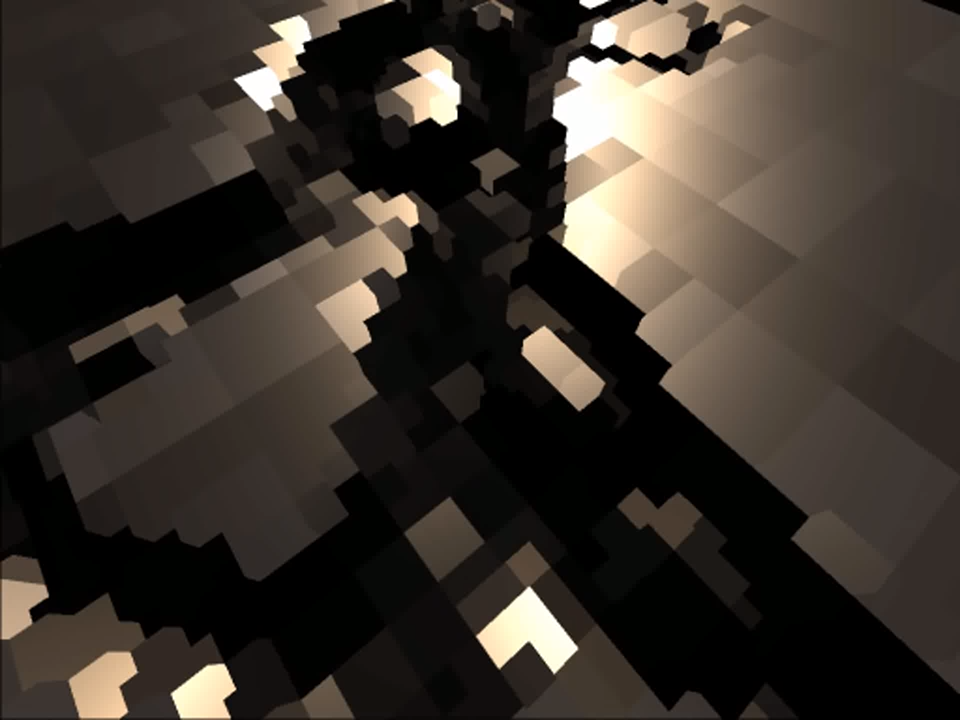
\includegraphics[width=200px]{graphics/newsoundgames_svo_coarse.png}
    \end{subfigure}%
    ~
    \begin{subfigure}{0.5\textwidth}
        \centering
        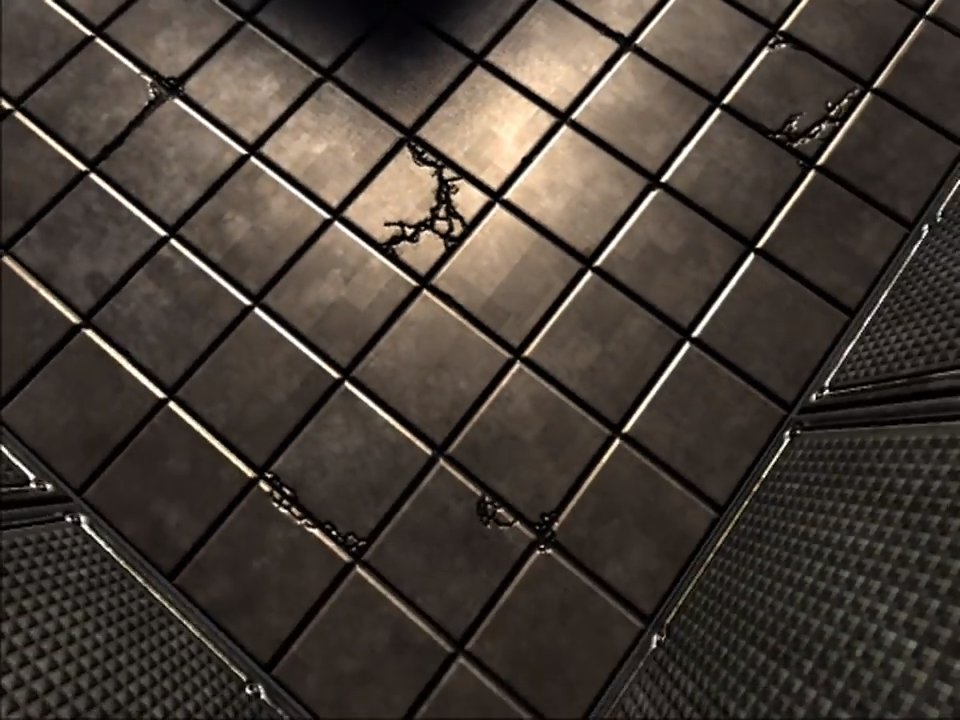
\includegraphics[width=200px]{graphics/newsoundgames_svo_fine.png}
    \end{subfigure}
    
    \caption{Two screenshots of a voxel engine by NewSoundGames\autocite{newsoundgames2012}. The image on the left shows a zoomed-in view of the floor crack shown in the rightmost image}
    \label{fig:voxel_details}
\end{figure}

By storing voxels in a space-efficient data structure, such as a Sparse Voxel Octree, it is possible to create highly detailed scenes. Figure \ref{fig:voxel_details} shows a voxel engine capable of representing surface detail at sub-millimetre precision. This paves the way for innovative software solutions beyond games; 3D modellers might use this technique to build very high resolution models, or medical imaging devices might use this technique to produce extremely detailed images.

Voxel ray-casting also comes with some desirable advantages. Since a ray is fired for every pixel on the screen, geometry which does not appear within the camera's field of view is never processed. This means that frustum culling is effectively free with ray casting. Ray-casting also belongs to a class of problems termed \textit{embarrassingly parallel}, meaning that it is a problem extremely well suited to parallelisation. This means that ray-casting is an excellent candidate for general-purpose GPU (GPGPU) programming. In this project, I utilise an OpenGL compute shader to perform the voxel rendering.

Finally, this project serves as an excellent vehicle to learn about modern high-performance rendering techniques and GPU programming; two areas of computer science that have always interested me.

\section{Objectives}
The overarching goal of this project is to produce a lightweight SDK that will allow  client developers to support very large, highly detailed virtual environments that can be edited in real-time. To achieve this, there are four main features that must be implemented:

\begin{enumerate}
    \item Support for extremely detailed scenes. I intend to support this feature through the use of specialised data structures for voxel storage (see Chapter \ref{chapter:voxel_data} for a discussion on voxel storage schemes). In concrete terms, the final artifact should be capable of rendering scenes to a voxel resolution of 1 millimetre.
    
    \item Support for very large scenes. Again, this feature is largely dependent on the choice of data structure for voxel storage.
    
    \item High performance. Fast rendering and responding quickly to user input is crucial in video games to maintain the illusion of fluid motion. Excluding client errors or exceptional circumstances (for example, the host machine does not support hardware accelerated rendering), \textit{Sabre} should complete all rendering operations within 33 milliseconds. This corresponds roughly to a frame-rate of thirty frames-per-second. Milliseconds-per-frame can be measured using Nvidia's Nsight graphics debugger (see section \ref{sec:tools}).
    
    \item Allow arbitrary modifications to the scene at run-time.
\end{enumerate}